%%%%%%%% ICML 2026 EXAMPLE LATEX SUBMISSION FILE %%%%%%%%%%%%%%%%%

\documentclass{article}

% Recommended, but optional, packages for figures and better typesetting:
\usepackage{microtype}
\usepackage{graphicx}
\usepackage{subcaption}
\usepackage{booktabs} % for professional tables

% hyperref makes hyperlinks in the resulting PDF.
% If your build breaks (sometimes temporarily if a hyperlink spans a page)
% please comment out the following usepackage line and replace
% \usepackage{icml2026} with \usepackage[nohyperref]{icml2026} above.
\usepackage{hyperref}


% Attempt to make hyperref and algorithmic work together better:
\newcommand{\theHalgorithm}{\arabic{algorithm}}

% Use the following line for the initial blind version submitted for review:
\usepackage{icml2026}

% For preprint, use
% \usepackage[preprint]{icml2026}

% If accepted, instead use the following line for the camera-ready submission:
% \usepackage[accepted]{icml2026}

\usepackage{amsmath}
\usepackage{amssymb}
\usepackage{mathtools}
\usepackage{amsthm}
\usepackage{algorithm}
\usepackage{algorithmic}

% TikZ for workflow figure
\usepackage{tikz}
\usetikzlibrary{shapes.geometric, arrows.meta, positioning, fit, backgrounds}

% if you use cleveref..
\usepackage[capitalize,noabbrev]{cleveref}

%%%%%%%%%%%%%%%%%%%%%%%%%%%%%%%%
% THEOREMS
%%%%%%%%%%%%%%%%%%%%%%%%%%%%%%%%
\theoremstyle{plain}
\newtheorem{theorem}{Theorem}[section]
\newtheorem{proposition}[theorem]{Proposition}
\newtheorem{lemma}[theorem]{Lemma}
\newtheorem{corollary}[theorem]{Corollary}
\theoremstyle{definition}
\newtheorem{definition}[theorem]{Definition}
\newtheorem{assumption}[theorem]{Assumption}
\theoremstyle{remark}
\newtheorem{remark}[theorem]{Remark}

% Todonotes is useful during development; simply uncomment the next line
%    and comment out the line below the next line to turn off comments
%\usepackage[disable,textsize=tiny]{todonotes}
\usepackage[textsize=tiny]{todonotes}

% The \icmltitle you define below is probably too long as a header.
% Therefore, a short form for the running title is supplied here:
\icmltitlerunning{CausalFlow: Generating Counterfactual Training Data for LLM Agent Post-Training}

\begin{document}

\twocolumn[
  \icmltitle{CausalFlow: Generating Counterfactual Training Data \\
    for LLM Agent Post-Training}

  % It is OKAY to include author information, even for blind submissions: the
  % style file will automatically remove it for you unless you've provided
  % the [accepted] option to the icml2026 package.

  % List of affiliations: The first argument should be a (short) identifier you
  % will use later to specify author affiliations Academic affiliations
  % should list Department, University, City, Region, Country Industry
  % affiliations should list Company, City, Region, Country

  % You can specify symbols, otherwise they are numbered in order. Ideally, you
  % should not use this facility. Affiliations will be numbered in order of
  % appearance and this is the preferred way.
  \icmlsetsymbol{equal}{*}

  \begin{icmlauthorlist}
    \icmlauthor{Anonymous Author 1}{inst}
    \icmlauthor{Anonymous Author 2}{inst}
  \end{icmlauthorlist}

  \icmlaffiliation{inst}{Anonymous Institution}

  \icmlcorrespondingauthor{Anonymous Author 1}{anonymous@institution.edu}

  % You may provide any keywords that you find helpful for describing your
  % paper; these are used to populate the "keywords" metadata in the PDF but
  % will not be shown in the document
  \icmlkeywords{LLM Agents, Synthetic Data Generation, Post-Training, Counterfactual Learning, Process Supervision, Machine Learning}

  \vskip 0.3in
]

% this must go after the closing bracket ] following \twocolumn[ ...

% This command actually creates the footnote in the first column listing the
% affiliations and the copyright notice. The command takes one argument, which
% is text to display at the start of the footnote. The \icmlEqualContribution
% command is standard text for equal contribution. Remove it (just {}) if you
% do not need this facility.

\printAffiliationsAndNotice{}  % leave empty for anonymous submission

\begin{abstract}
High-quality training data for LLM agents remains scarce because it requires multi-step reasoning traces with tool use and environment interaction, while most synthetic pipelines produce only successful trajectories or uninformative failures.
We introduce \textsc{CausalFlow}, a data generation framework that transforms agent failures into contrastive supervision by pairing each failed execution with a minimally edited counterfactual repair.
\textsc{CausalFlow} formalizes an agent trace as a dependency DAG and performs step-level interventional attribution to identify failure-inducing steps via \emph{Causal Responsibility Scores} (CRS): a step is responsible if intervening on it and re-executing downstream steps flips the outcome to the correct answer.
Conditioned on CRS-positive steps, we generate multiple repair candidates and select those that are both \emph{validated} (they succeed under re-execution or outcome verification) and \emph{minimal} (high token-overlap edits).
Across four benchmarks spanning math (GSM8K), code (MBPP), web QA (SealQA Hard), and medical browsing (MedBrowseComp), \textsc{CausalFlow} converts 42.7\% of failed runs (555/1299) into validated (failed\_trace, repaired\_trace) pairs, achieving minimality scores of 0.79--0.87 (see \Cref{tab:main_results}).
The generated dataset includes step-level causal annotations and skill taxonomy labels that support process supervision and curriculum learning, providing a scalable path for agent post-training from real failure traces.
\end{abstract}

\section{Introduction}

LLM-powered agents have emerged as a promising paradigm for autonomous problem-solving, combining language model reasoning with tool use, memory access, and environmental interaction \cite{yao2023react,schick2023toolformer,nakano2021webgpt}. However, training agents to perform complex multi-step tasks remains challenging due to a fundamental data scarcity problem: high-quality training data for agentic capabilities is expensive to collect and difficult to generate synthetically.

Current approaches to agent training face three key limitations. First, agentic training data requires multi-step reasoning traces with tool use, which are expensive to manually annotate at scale. Second, typical synthetic generation methods lack error correction signals as they produce either successful traces or failed traces, but not paired examples showing what went wrong and how to fix it. Third, existing data lacks step-level supervision; annotations indicate only whether the final outcome was correct, not which intermediate steps caused failures.

We propose a novel perspective: \emph{agent failures are a rich source of training data, not just evaluation artifacts}. Every failed execution, when paired with a targeted repair, becomes a contrastive training example. The key is identifying \emph{which} steps to repair and generating \emph{minimal} corrections that teach precise fixes rather than wholesale rewrites.

We introduce \textsc{CausalFlow}, a pipeline for generating high-quality contrastive training data from agent failures. Given a failed execution, \textsc{CausalFlow}:
\begin{enumerate}
    \item Constructs a \textbf{causal graph} from explicit step dependencies
    \item Computes \textbf{Causal Responsibility Scores} (CRS) to identify which steps caused the failure
    \item Generates \textbf{minimal counterfactual repairs} that fix only the causal steps
\end{enumerate}

\begin{figure}[t]
\centering
\resizebox{\columnwidth}{!}{%
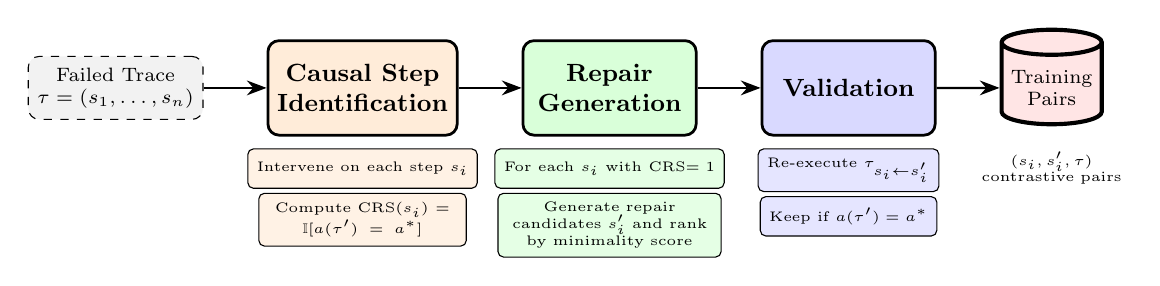
\begin{tikzpicture}[
    node distance=0.6cm and 0.8cm,
    mainbox/.style={rectangle, draw, rounded corners, minimum height=1.2cm, minimum width=2.2cm, align=center, font=\small\bfseries, line width=1pt},
    subbox/.style={rectangle, draw, rounded corners=2pt, minimum height=0.5cm, minimum width=2.2cm, align=center, font=\tiny},
    inputbox/.style={rectangle, draw, rounded corners, minimum height=0.8cm, minimum width=1.6cm, align=center, font=\scriptsize, dashed},
    % --- CB: Changed style to database cylinder ---
    outputbox/.style={cylinder, shape border rotate=90, draw, minimum height=1.2cm, minimum width=1.2cm, shape aspect=0.25, align=center, font=\scriptsize, line width=1.5pt},
    % ----------------------------------------------
    arrow/.style={-{Stealth[length=2.5mm]}, thick},
    note/.style={font=\tiny, align=center},
    label/.style={font=\tiny\itshape, text=gray},
]
    % Input
    \node[inputbox, fill=gray!10] (input) {Failed Trace\\$\tau = (s_1, \ldots, s_n)$};
    
    % Stage 1: Causal Step Identification
    \node[mainbox, fill=orange!15, right=of input] (crs) {Causal Step\\Identification};
    \node[subbox, fill=orange!10, below=0.15cm of crs] (crs1) {Intervene on each step $s_i$};
    \node[subbox, fill=orange!10, below=0.05cm of crs1, text width=2.4cm] (crs2) {Compute CRS$(s_i) = \mathbb{I}[a(\tau') = a^*]$};
    
    % Stage 2: Repair Generation
    \node[mainbox, fill=green!15, right=of crs] (repair) {Repair\\Generation};
    \node[subbox, fill=green!10, below=0.15cm of repair] (rep1) {For each $s_i$ with CRS$=1$};
    \node[subbox, fill=green!10, below=0.05cm of rep1, text width=2.6cm] (rep2) {Generate repair candidates $s'_i$ and rank by minimality score};
    
    % Stage 3: Validation
    \node[mainbox, fill=blue!15, right=of repair] (validate) {Validation};
    \node[subbox, fill=blue!10, below=0.15cm of validate] (val1) {Re-execute $\tau_{s_i \leftarrow s'_i}$};
    \node[subbox, fill=blue!10, below=0.05cm of val1] (val2) {Keep if $a(\tau') = a^*$};
    
    % Output (Database shape applied here)
    \node[outputbox, fill=red!10, right=of validate] (output) {Training\\Pairs};
    
    % Main arrows
    \draw[arrow] (input) -- (crs);
    \draw[arrow] (crs) -- (repair);
    \draw[arrow] (repair) -- (validate);
    \draw[arrow] (validate) -- (output);
    
    % Output description
    \node[note, below=0.2cm of output, text width=1.8cm] (outnote) {$(s_i, s'_i, \tau)$\\contrastive pairs};
    
\end{tikzpicture}
}
\caption{Overview of the CausalFlow pipeline.}
\label{fig:pipeline}
\end{figure}

Our key insight is that counterfactual repairs provide contrastive supervision: models see both the incorrect reasoning and the corrected version for the same problem. This paired structure, combined with step-level causal annotations, enables more targeted learning than training on successful traces alone. \Cref{fig:pipeline} illustrates the complete pipeline.

We evaluate \textsc{CausalFlow} on four diverse benchmarks spanning mathematical reasoning (GSM8K), code generation (MBPP), question answering (SealQA Hard), and medical web browsing (MedBrowseComp), totaling over 3{,}000 problems. Our pipeline converts 42.7\% of failures into validated training pairs with high minimality scores (0.79--0.87). We also organize generated data by a skill taxonomy of 12--16 categories per domain, enabling curriculum-based training.

\paragraph{Contributions.} Our main contributions are:
\begin{itemize}
    \item A pipeline for automatically generating contrastive (failed trace, repaired step) training pairs from agent execution failures (and repaired traces when deterministic re-execution is available)
    \item Step-level causal annotations via Causal Responsibility Scores (CRS) that identify exactly which steps to learn from
    \item Quality signals for generated data through minimality constraints on causal attributions
    \item Extensive experiments across over 3{,}000 problems converting 42.7\% of failures into validated training pairs, with analysis of data quality metrics and skill taxonomies
\end{itemize}

While our motivation is agent post-training, this work focuses on \emph{data generation and quality analysis}; evaluating downstream training improvements from \textsc{CausalFlow}-generated data is left for future work.


\section{Related Work}

\paragraph{Synthetic Data for LLM Training.}
Generating synthetic training data has become essential for LLM development. Self-Instruct \cite{wang2023selfinstruct} generates instruction-following data from seed examples. RLHF pipelines \cite{ouyang2022training} create preference data through human feedback. Rejection sampling approaches \cite{yuan2023scaling} filter model outputs for quality. Constitutional AI \cite{bai2022constitutional} uses self-critique to generate preference pairs. However, these methods focus on single-turn or simple multi-turn settings, not complex agentic traces with tool use. \textsc{CausalFlow} addresses this gap by generating contrastive training pairs specifically from agent execution failures.

\paragraph{Process Supervision.}
Recent work has shown that step-level supervision improves reasoning capabilities. Process reward models \cite{lightman2023lets} train verifiers on human-annotated step correctness. Outcome vs.\ process supervision \cite{uesato2022solving} demonstrates benefits of intermediate feedback. However, obtaining step-level labels is expensive. \textsc{CausalFlow} automatically generates step-level annotations through causal attribution, identifying which steps caused failures without human labeling.

\paragraph{Causal Inference in Machine Learning.}
Causal inference provides tools for understanding interventional effects and counterfactual reasoning \cite{pearl2009causality,peters2017elements}. Applications to ML interpretability include causal feature attribution \cite{schwab2019cxplain}, causal concept explanations \cite{goyal2019explaining}, and causal tracing in transformers \cite{meng2022locating}. Our work extends these ideas to the structured domain of agent execution traces, where explicit step dependencies enable direct causal graph construction. We use causal attribution not for explanation but for \emph{data generation}: identifying which steps to repair to create training pairs.

\paragraph{Error Analysis and Self-Correction.}
Prior work has analyzed LLM errors through behavioral testing \cite{ribeiro2020beyond} or chain-of-thought analysis \cite{wei2022chain}. Self-debugging approaches \cite{chen2024teaching} have models fix their own errors but lack principled identification of which steps to fix. Our CRS-based approach provides formal grounding for identifying causal steps, enabling targeted repair generation rather than wholesale trace rewriting.

\section{Preliminaries}

\subsection{Agent Execution Traces}

We model an LLM agent execution as a sequence of typed steps $\tau = (s_1, s_2, \ldots, s_n)$, where each step $s_i$ has:
\begin{itemize}
    \item A \textbf{type} $t_i \in \mathcal{T}$, where $\mathcal{T} = \{\texttt{reasoning}, \texttt{tool\_call}, \texttt{tool\_response},$ \\ $\texttt{llm\_response}, \texttt{memory\_access}, \\ \texttt{environment\_action},$ \\ $\texttt{environment\_observation}, \texttt{final\_answer}\}$
    \item Type-specific \textbf{content} (e.g., reasoning text, tool name and arguments, or observation data)
    \item A set of \textbf{dependencies} $D_i \subseteq \{1, \ldots, i-1\}$ indicating which prior steps $s_i$ directly depends on
\end{itemize}

The final step is always of type \texttt{final\_answer} and represents the agent's output. We denote the agent's final answer as $a(\tau)$ and the ground truth as $a^*$. An execution is \emph{successful} if $a(\tau) = a^*$ and \emph{failed} otherwise.

\subsection{Causal Graphs from Traces}

The dependencies $D_i$ naturally induce a directed acyclic graph (DAG) $G = (V, E)$ where $V = \{s_1, \ldots, s_n\}$ and $(s_j, s_i) \in E$ iff $j \in D_i$. This \emph{causal graph} represents the causal structure of the execution: $s_i$ causally depends on its ancestors in $G$.
In many agent traces this structure is close to linear, but explicit dependencies still provide a principled way to scope local context and downstream effects during interventions, and they generalize to agents with branching tool use or explicit state.

\begin{definition}[Causal Ancestors]
For step $s_i$, the causal ancestors $\text{Anc}(s_i)$ are all steps reachable by following edges backwards from $s_i$. These are the steps that could potentially influence $s_i$.
\end{definition}

\begin{definition}[Causal Steps]
The set of causal steps for a failed trace $\tau$ is 
$\mathcal{C}(\tau) = \{s_i : \text{CRS}(s_i) = 1\}$, 
containing all steps where intervention leads to successful outcome. 
These are the candidate steps for repair generation.
\end{definition}

\begin{definition}[Contrastive Training Pair]
A contrastive training pair $(s_i, s_i', \tau)$ consists of an original failed 
step $s_i$, its validated repair $s_i'$, and the failed trace context $\tau$. 
When deterministic re-execution is available, we additionally include the 
repaired trace $\tau_{s_i \leftarrow s_i'}$.
\end{definition}


\section{The CausalFlow Pipeline}

We now present the \textsc{CausalFlow} pipeline for generating training data from agent failures. The pipeline has four components: capturing agent behavior, identifying teachable moments through causal attribution, generating contrastive training pairs, and validating data quality.

\subsection{Capturing Agent Behavior}

The first stage captures detailed execution traces from agent runs. These traces form the raw material from which training data is generated. Failed traces (where $a(\tau) \neq a^*$) are candidates for training pair generation, as each failure represents an opportunity to create a contrastive example.

\subsection{Identifying Teachable Moments}

Not every step in a failed trace is worth learning from. Our goal is to identify which steps are \emph{causally responsible} for the failure these are the ``teachable moments'' where targeted corrections provide the most training signal. We adopt an interventionist approach inspired by actual causation \cite{halpern2005causes}: a step is causally responsible if intervening on it would change the outcome.

\begin{definition}[Causal Responsibility Score]
For a failed trace $\tau$ with outcome $a(\tau) \neq a^*$, the \emph{Causal Responsibility Score} of step $s_i$ is:
\begin{equation}
    \text{CRS}(s_i) = \mathbb{I}\left[ a(\tau_{s_i \leftarrow s_i'}) = a^* \right]
\end{equation}
where $\tau_{s_i \leftarrow s_i'}$ denotes the trace obtained by replacing $s_i$ with an intervened version $s_i'$ and re-executing all subsequent steps, and $\mathbb{I}[\cdot]$ is the indicator function.
\end{definition}

Intuitively, $\text{CRS}(s_i) = 1$ if fixing step $s_i$ (while propagating effects forward) leads to a successful outcome. This provides a binary measure of causal responsibility.

\paragraph{Computing Interventions.}
To compute $s_i'$, we prompt an LLM with the original step $s_i$, a small context window over its explicit dependencies (e.g., the most recent dependent steps), and feedback about the execution failure. The LLM generates a ``corrected'' version of the step. For reasoning steps, this corrects logical errors; for tool calls, this fixes incorrect arguments or tool selection.

\paragraph{Re-execution.}
After intervention on $s_i$, we re-execute the trace from step $i+1$ onwards. This can be done either:
\begin{itemize}
    \item \textbf{Deterministically}: If a domain-specific executor is available (e.g., Python interpreter for code), we re-run the actual computation
    \item \textbf{Predictively}: We use an LLM to predict whether the intervened trace would succeed, based on the corrected step and original context
\end{itemize}

\Cref{alg:crs} summarizes the CRS computation.

\begin{algorithm}[tb]
   \caption{Causal Responsibility Scoring}
   \label{alg:crs}
\begin{algorithmic}
   \STATE {\bfseries Input:} Failed trace $\tau = (s_1, \ldots, s_n)$, gold answer $a^*$
   \STATE {\bfseries Output:} CRS scores $\{\text{CRS}(s_i)\}_{i=1}^{n-1}$
   \FOR{$i = 1$ {\bfseries to} $n-1$}
   \STATE $s_i' \leftarrow \text{GenerateIntervention}(s_i, \text{DepContext}(s_i), \text{feedback})$
   \IF{$s_i' = \varnothing$}
   \STATE $\text{CRS}(s_i) \leftarrow 0$ \COMMENT{No intervention generated}
   \ELSE
   \STATE $\tau' \leftarrow \text{ReExecuteOrPredict}(\tau, i, s_i')$
   \STATE $\text{CRS}(s_i) \leftarrow \mathbb{I}[a(\tau') = a^*]$
   \ENDIF
   \ENDFOR
   \STATE {\bfseries return} $\{\text{CRS}(s_i)\}$
\end{algorithmic}
\end{algorithm}

\subsection{Generating Contrastive Training Pairs}

For steps with $\text{CRS}(s_i) = 1$ (i.e., causally responsible steps), we generate \emph{counterfactual repairs} i.e minimal step-level modifications that, combined with the original failed trace, form contrastive training pairs. In domains where deterministic re-execution is available, we can additionally re-run the agent from the repaired step to obtain a repaired trace; otherwise we retain the repaired step and validate via outcome prediction.

\paragraph{Minimality for Training Quality.}
A key desideratum is that repairs should be \emph{minimal}: they should fix only the identified error without introducing unnecessary changes. Minimal repairs ensure models learn targeted corrections rather than wholesale rewrites, making the training signal more precise. We define minimality as:
\begin{equation}
    \text{Minimality}(s_i, s_i') =
    \frac{m}{L}\left(1 - \tfrac{1}{2}\cdot\frac{\left|\;|x|-|y|\;\right|}{L}\right),
\end{equation}
where $x=\text{tokens}(s_i)$ and $y=\text{tokens}(s_i')$ are token \emph{sequences}, $L=\max(|x|,|y|)$, and $m=\sum_{k=1}^{\min(|x|,|y|)} \mathbb{I}[x_k = y_k]$ counts position-wise token matches. Higher scores indicate smaller edits.

\paragraph{Repair Generation.}
We generate multiple repair proposals per causal step using temperature sampling, then rank by minimality. The repair prompt emphasizes:
\begin{enumerate}
    \item Fixing the \emph{logical error} in the specific step
    \item Not using the gold answer directly
    \item Making the smallest possible change
\end{enumerate}

Each repair is validated by re-execution (deterministic) or outcome prediction (LLM-based) to confirm it leads to success. Successfully validated pairs are added to the training dataset.

\subsection{Training Data Properties}

The resulting training data has several properties valuable for agent post-training:

\paragraph{Contrastive Pairs.} Each training example contains the failed trace and a minimally repaired version of a causally responsible step. When deterministic re-execution is available, we also include the repaired trace obtained by re-running the agent forward from the repaired step; otherwise the repaired trace is not materialized and we use outcome prediction for validation. This contrastive structure enables models to learn from explicit comparisons between incorrect and corrected behavior.

\paragraph{Step-Level Annotations.} CRS provides binary labels indicating which steps caused the failure. This enables process supervision so models can receive feedback at individual steps, not just final outcomes.

\paragraph{Minimal Edits.} By ranking repairs by minimality, training pairs teach targeted corrections. Models learn precise fixes rather than learning to completely rewrite traces.

\paragraph{Skill Taxonomy.} We cluster labeled causal steps by their error patterns to organize analysis (and optionally training data selection) into skill categories (e.g., arithmetic errors, loop logic bugs, query formulation issues). In our codebase this is implemented as a separate post-processing step over stored traces and analyses.


\section{Experiments}

We evaluate \textsc{CausalFlow} on four diverse benchmarks to answer:
\begin{enumerate}
    \item[\textbf{Q1}] How much training data can \textsc{CausalFlow} generate from agent failures?
    \item[\textbf{Q2}] What is the quality of generated training pairs (minimality, repair rate)?
    \item[\textbf{Q3}] What skill categories does the generated data cover?
\end{enumerate}

\subsection{Experimental Setup}

\paragraph{Benchmarks.}
We evaluate on four benchmarks spanning different domains (see \Cref{tab:benchmark_setup} for full details):
\begin{itemize}
    \item \textbf{GSM8K} \cite{cobbe2021gsm8k}: Grade school math word problems requiring multi-step arithmetic reasoning
    \item \textbf{MBPP} \cite{austin2021program}: Python programming problems from the Mostly Basic Programming Problems benchmark
    \item \textbf{SealQA Hard} \cite{pham2025sealqa}: Complex question answering requiring web search and synthesis
    \item \textbf{MedBrowseComp} \cite{chen2025medbrowsecomp}: Medical question answering with web browsing capabilities
\end{itemize}

\paragraph{Agent Setup.}
For each benchmark, we run an appropriate LLM agent:
\begin{itemize}
    \item GSM8K: Gemini 2.0 Flash Lite with calculator tool
    \item MBPP: GPT-5 Chat with Docker-based Python execution
    \item SealQA Hard: Gemini 3 Flash with web search
    \item MedBrowseComp: Gemini 3 Flash with web browsing
\end{itemize}

\paragraph{Metrics.}
We report:
\begin{itemize}
    \item \textbf{Repair Success Rate}: Fraction of failed executions converted into validated training pairs (this directly measures the pipeline's utility for training data generation)
    \item \textbf{Minimality Score}: Average minimality between original and repaired steps (higher = smaller edits)
    \item \textbf{Skill Groups}: Number of distinct skill categories in generated data
\end{itemize}

% Benchmark setup table
\begin{table}[t]
  \caption{Benchmark setup details. All experiments use the same \textsc{CausalFlow} pipeline with domain-specific validation methods.}
  \label{tab:benchmark_setup}
  \centering
  \begin{small}
    \begin{sc}
      \begin{tabular}{lcc}
        \toprule
        Benchmark & Model & Validation \\
        \midrule
        GSM8K & Gemini 2.0 & LLM predict\\
        MBPP & GPT-5 Chat & Docker exec \\
        SealQA & Gemini 3 Flash & Re-execution \\
        MedBrowseComp & Gemini 3 Flash & Re-execution\\
        \bottomrule
      \end{tabular}
    \end{sc}
  \end{small}
\end{table}

\subsection{Training Data Generation Results}

\Cref{tab:main_results} presents training data generation results across all benchmarks.

\begin{table}[t]
  \caption{Training data generation results. \textsc{CausalFlow} converts 42.7\% of failures into validated training pairs across four benchmarks. Failed = number of failed agent executions; Pairs = validated (failed, repaired) training pairs generated; Rate = repair success rate (Pairs/Failed); Min.\ = average minimality score.}
  \label{tab:main_results}
  \centering
  \begin{small}
    \begin{sc}
      \begin{tabular}{lcccc}
        \toprule
        Benchmark & Failed & Pairs & Rate & Min. \\
        \midrule
        GSM8K        & 330 & 173 & 52.4\% & 0.87 \\
        MBPP         & 488 & 201 & 41.2\% & 0.82 \\
        SealQA Hard  & 146 & 32  & 21.9\% & 0.79 \\
        MedBrowseComp& 335 & 149 & 44.5\% & 0.84 \\
        \midrule
        \textbf{Total} & 1299 & 555 & 42.7\% & 0.83 \\
        \bottomrule
      \end{tabular}
    \end{sc}
  \end{small}
\end{table}

\textsc{CausalFlow} achieves its highest repair success rate on GSM8K (52.4\%), where errors tend to be localized arithmetic or reasoning mistakes amenable to minimal repair. GSM8K also achieves the highest minimality score (0.87). The lowest rate is on SealQA Hard (21.9\%), where failures often involve information retrieval gaps that cannot be fixed by modifying reasoning steps alone.

\paragraph{Training Pair Characteristics.}
Generated training pairs exhibit several patterns:
\begin{itemize}
    \item \textbf{Arithmetic corrections} (GSM8K): Pairs showing incorrect $\rightarrow$ correct calculation steps
    \item \textbf{Logic bug fixes} (MBPP): Pairs demonstrating off-by-one error corrections, boundary condition handling
    \item \textbf{Query refinement} (SealQA, MedBrowseComp): Pairs showing improved search query formulation
    \item \textbf{Reasoning corrections}: Pairs fixing incorrect inferences or missed constraints
\end{itemize}

\subsection{Skill Taxonomy for Curriculum Learning}

\textsc{CausalFlow}'s causal attributions reveal skill categories that organize generated training data. We cluster causal steps by their error patterns to create a skill taxonomy, enabling curriculum-based training (\Cref{tab:skills}). GSM8K has the most diverse categories (16), including arithmetic operations, unit conversions, multi-step planning, and constraint tracking. MBPP clusters into 12 categories covering loop logic, string manipulation, and edge case handling. This taxonomy enables targeted training: practitioners can select training pairs for specific skills their models struggle with, or construct curricula progressing from simpler to more complex skill categories.

\subsection{Qualitative Examples}

\paragraph{Example 1: Off-by-One Error in Break-Even Analysis.}
Consider this problem from GSM8K: ``Carlos is planting a lemon tree. The tree will cost \$90 to plant. Each year it will grow 7 lemons, which he can sell for \$1.5 each. It costs \$3 a year to water and feed the tree. How many years will it take before he starts earning money on the lemon tree?''

The agent trace shows:
\begin{enumerate}
    \item Reasoning: ``Calculate annual income: 7 lemons $\times$ \$1.5 = \$10.50''
    \item Tool call: \texttt{calculator(7 * 1.5) = 10.5}
    \item Reasoning: ``Calculate net profit per year: \$10.50 $-$ \$3 = \$7.50''
    \item Tool call: \texttt{calculator(10.5 - 3) = 7.5}
    \item Reasoning: ``Years to cover initial cost: \$90 $\div$ \$7.50 = 12''
    \item Tool call: \texttt{calculator(90 / 7.5) = 12}
    \item Final answer: 12 [INCORRECT: gold answer is 13]
\end{enumerate}

The error is subtle: 12 years of \$7.50 profit exactly covers the \$90 cost (break-even), but the question asks when Carlos \emph{starts earning money} i.e., when cumulative profit first becomes \emph{positive}, not zero. At year 13, he has his first positive earnings.

\textsc{CausalFlow} identifies Step 5 as causal and generates the validated repair: ``\ldots Divide the initial cost by the annual net profit to find the number of years. Since we are looking for when he \emph{starts} earning money i.e., when cumulative profit \emph{first} becomes positive, if the division results in a whole number, we need to add one year.''

\paragraph{Training Value.} This contrastive pair teaches models to distinguish break-even from positive-profit conditions, a common off-by-one reasoning error. The repair targets the planning step where the boundary condition was missed rather than simply changing the final answer.

\paragraph{Example 2: MBPP Logic Bug.}
A function to check if a number is prime incorrectly returns \texttt{True} for 1:
\begin{verbatim}
def is_prime(n):
    for i in range(2, n):
        if n % i == 0:
            return False
    return True  # Bug: n=1 returns True
\end{verbatim}

\textsc{CausalFlow} traces the failure to the missing base case and generates a minimal repair adding \texttt{if n <= 1: return False}.

\paragraph{Training Value.} This pair teaches edge case handling: the original trace shows the common pattern of forgetting boundary conditions, and the repair demonstrates the minimal fix. The contrastive structure helps models learn to check base cases when implementing mathematical predicates.

\subsection{Ablation Studies}

\paragraph{Minimality Constraint.}
Without minimality ranking, repairs tend to involve larger rewrites. While these repairs still lead to correct answers, they provide a weaker training signal because models learn to rewrite traces rather than make targeted fixes. The minimality constraint ensures training pairs teach precise corrections.

\begin{table}[t]
  \caption{Skill taxonomy for generated training data. Numbers indicate distinct categories for organizing training pairs by skill deficit. Categories are derived from clustering causal steps by error patterns.}
  \label{tab:skills}
  \centering
  \begin{small}
    \begin{sc}
      \begin{tabular}{lcc}
        \toprule
        Benchmark & Skills & Example Categories \\
        \midrule
        GSM8K & 16 & arithmetic, unit conv. \\
        MBPP & 12 & loop logic, strings \\
        SealQA Hard & 4 & query, synthesis \\
        MedBrowseComp & 6 & med.\ reasoning \\
        \bottomrule
      \end{tabular}
    \end{sc}
  \end{small}
\end{table}

\section{Discussion}

\paragraph{Key Findings.}
Our experiments reveal several insights about generating training data from agent failures:
\begin{enumerate}
    \item \textbf{Failures are often localized}: In most cases, 1--3 steps are causally responsible, enabling targeted training pairs rather than wholesale trace rewrites
    \item \textbf{Generation rates vary by domain}: Closed-domain tasks (GSM8K, MBPP) yield higher-quality training data than open-domain retrieval tasks
    \item \textbf{Skill taxonomies emerge}: Causal analysis naturally organizes training data into interpretable skill categories for curriculum learning
\end{enumerate}

\paragraph{Implications for Agent Training.}
The contrastive training pairs generated by \textsc{CausalFlow} enable several training approaches:
\begin{itemize}
    \item \textbf{Process supervision}: Step-level CRS annotations provide supervision signal at intermediate steps, not just final outcomes
    \item \textbf{Curriculum learning}: Skill taxonomies enable training curricula that target specific capability gaps
    \item \textbf{Contrastive learning}: (Failed, repaired) pairs can train models to distinguish correct from incorrect reasoning
    \item \textbf{Self-improvement}: Models can be trained on repairs of their own failures, creating a closed-loop improvement cycle
\end{itemize}

\paragraph{Limitations.}
\textsc{CausalFlow} has several limitations:
\begin{itemize}
    \item \textbf{Repair quality}: LLM-generated repairs may not always represent optimal fixes; we validate repairs via deterministic re-execution when available or LLM-based outcome prediction otherwise
    \item \textbf{Generation costs}: Computing CRS requires re-running (parts of) traces, which can be expensive for complex agents
    \item \textbf{Retrieval failures}: When failures stem from information not being retrievable (vs.\ reasoning errors), useful training pairs cannot be generated
    \item \textbf{Coverage}: Not all agent failures can be converted to training pairs; some require architectural changes rather than step repairs
\end{itemize}

\paragraph{Future Work.}
Promising directions include: (1) training agents on \textsc{CausalFlow}-generated data to measure downstream improvement, (2) active learning to prioritize failure cases most valuable for training, (3) extending to multi-agent systems where failures involve coordination, and (4) learning to predict CRS without re-execution to reduce generation costs.


\section{Conclusion}

We presented \textsc{CausalFlow}, a pipeline for generating high-quality contrastive training data from LLM agent failures. By applying causal inference to identify which steps caused failures and generating minimal counterfactual repairs, \textsc{CausalFlow} transforms agent failures into (failed trace, repaired step) training pairs (and repaired traces when deterministic re-execution is available). Experiments on four benchmarks (over 3{,}000 total problems) demonstrate that \textsc{CausalFlow} converts 42.7\% of failures into validated training pairs with high minimality scores (0.79--0.87), as shown in \Cref{tab:main_results}. The repair success rate directly measures the pipeline's utility: each validated pair represents a failure successfully converted into contrastive supervision. The dataset includes step-level causal annotations, and we additionally derive skill taxonomies for curriculum learning via post-processing (\Cref{tab:skills}). We believe automated generation of contrastive training data from failures is a promising direction for scalable agent post-training.


\section*{Impact Statement}

This paper presents work whose goal is to advance the field of Machine Learning, specifically in generating training data for improving LLM agent capabilities. \textsc{CausalFlow} enables practitioners to automatically generate high-quality training data from agent failures, potentially reducing the cost and effort required to improve agent systems.

The generated training data could be used to make agents more capable, which has both positive applications (more reliable AI assistants) and potential risks (more capable systems may be misused). We believe the benefits of improved agent training outweigh these risks, as the same training improvements could be achieved through more expensive manual annotation. Our work reduces costs but does not enable fundamentally new capabilities.


\bibliography{causalflow_data_gen}
\bibliographystyle{icml2026}

%%%%%%%%%%%%%%%%%%%%%%%%%%%%%%%%%%%%%%%%%%%%%%%%%%%%%%%%%%%%%%%%%%%%%%%%%%%%%%%
%%%%%%%%%%%%%%%%%%%%%%%%%%%%%%%%%%%%%%%%%%%%%%%%%%%%%%%%%%%%%%%%%%%%%%%%%%%%%%%
% APPENDIX
%%%%%%%%%%%%%%%%%%%%%%%%%%%%%%%%%%%%%%%%%%%%%%%%%%%%%%%%%%%%%%%%%%%%%%%%%%%%%%%
%%%%%%%%%%%%%%%%%%%%%%%%%%%%%%%%%%%%%%%%%%%%%%%%%%%%%%%%%%%%%%%%%%%%%%%%%%%%%%%
\newpage
\appendix
\onecolumn

\section{Experimental Details}
\label{app:experimental_details}

This section provides complete experimental setup details for each benchmark, including dataset specifications, agent configurations, prompts used, and validation methods.

\subsection{GSM8K}
\label{app:gsm8k}

\paragraph{Dataset.}
We use the GSM8K dataset \cite{cobbe2021gsm8k} loaded from HuggingFace (\texttt{gsm8k}, \texttt{main} config, \texttt{test} split), comprising 1,319 grade-school math word problems.

\paragraph{Model.}
\begin{itemize}
    \item \texttt{model\_used}: \texttt{google/gemini-2.0-flash-lite-001}
    \item Temperature: 0.7
\end{itemize}

\paragraph{Agent Configuration.}
The GSM8K agent (\texttt{GSM8KAgent}) decomposes problems into structured steps:
\begin{enumerate}
    \item Initial reasoning step stating the problem
    \item LLM generates structured solution with reasoning, steps (each with description, operation, expression), and final answer
    \item For each calculation step: reasoning $\rightarrow$ calculator tool call $\rightarrow$ tool response
    \item Final answer step
\end{enumerate}

\paragraph{Tools.}
\begin{itemize}
    \item \texttt{calculator}: Evaluates mathematical expressions using \texttt{MathReexecutor}
\end{itemize}

\paragraph{Prompts.}
The solve prompt requests:
\begin{verbatim}
Solve this math problem step by step.
Problem: {question}
Provide:
1. A brief reasoning about your approach
2. Each calculation step with:
   - A clear description
   - The operation type (addition, subtraction, multiplication, division, or other)
   - The exact mathematical expression to evaluate
3. The final numerical answer
Be precise with expressions - they should be evaluatable.
\end{verbatim}

\paragraph{Validation Method.}
LLM-based outcome prediction (no deterministic re-executor). Gold answers are extracted as numeric values using \texttt{MathReexecutor.extract\_number()}.

\paragraph{CausalFlow Configuration.}
\begin{itemize}
    \item Intervene on step types: \texttt{TOOL\_CALL}, \texttt{LLM\_RESPONSE}, \texttt{REASONING}, \texttt{TOOL\_RESPONSE}
\end{itemize}

\subsection{MBPP}
\label{app:mbpp}

\paragraph{Dataset.}
We use the MBPP dataset \cite{austin2021program} loaded from HuggingFace (\texttt{Muennighoff/mbpp}), with train/test/validation/prompt splits merged. Total problems: 974 (after filtering).

\paragraph{Model.}
\begin{itemize}
    \item \texttt{model\_used}: GPT 5 Chat
    \item Temperature: 0.2 for code generation
\end{itemize}

\paragraph{Agent Configuration.}
The MBPP agent reuses the HumanEval-style code generator (\texttt{HumanevalAgent}):
\begin{enumerate}
    \item Reasoning step: ``Implement \{function\} for task \{id\}''
    \item Tool call: \texttt{llm\_code\_generation}
    \item LLM response: generated Python code
    \item Tool call: \texttt{docker\_code\_execution}
    \item Tool response: test results
    \item Final answer: ``pass'' or ``fail''
\end{enumerate}

\paragraph{Tools.}
\begin{itemize}
    \item \texttt{llm\_code\_generation}: Generates Python code via LLM
    \item \texttt{docker\_code\_execution}: Runs code in isolated Docker container with official test cases
\end{itemize}

\paragraph{Prompts.}
Code generation prompt:
\begin{verbatim}
Complete the following Python function. Return only executable Python code.
{prompt}

Rules:
- Function name must be exactly `{entry_point}`
- Preserve provided signature and docstring
- Include required imports
- No extra prints or explanations
\end{verbatim}

\paragraph{Validation Method.}
Deterministic Docker-based execution using \texttt{HumanevalReexecutor}. Tests are run in isolated containers; success requires all test assertions to pass.

\paragraph{CausalFlow Configuration.}
\begin{itemize}
    \item Deterministic re-executor: \texttt{HumanevalReexecutor} with Docker
\end{itemize}

\subsection{SealQA Hard}
\label{app:sealqa}

\paragraph{Dataset.}
We use SealQA Hard \cite{pham2025sealqa} loaded from HuggingFace (\texttt{vtllms/sealqa}, \texttt{seal\_hard} config, \texttt{test} split), comprising 254 complex QA problems requiring web search.

\paragraph{Model.}
\begin{itemize}
    \item \texttt{model\_used}: \texttt{google/gemini-3-flash-preview}
    \item Temperature: 0.0 for solver, 0.3 for agent steps
\end{itemize}

\paragraph{Agent Configuration.}
The BrowseComp agent (\texttt{BrowseCompAgent}) uses a structured tool policy:
\begin{itemize}
    \item Maximum steps: 15
    \item Actions: \texttt{search}, \texttt{open\_url}, \texttt{extract}, \texttt{answer}
    \item State tracking: gathered facts, search history, page summaries
\end{itemize}

\paragraph{Tools.}
\begin{itemize}
    \item \texttt{web\_search}: Search via Serper API with caching
    \item \texttt{web\_fetch}: Fetch and parse web pages
\end{itemize}

\paragraph{Prompts.}
Agent system prompt:
\begin{verbatim}
You are a web browsing agent tasked with answering questions 
by searching the web and examining pages.

You have access to the following tools:
1. search(query) - Search the web for information
2. open_url(url) - Fetch and read the content of a specific URL
3. extract - Note important facts from the current context
4. answer - Provide your final answer when you have enough information

Important guidelines:
- Start by searching for relevant information
- Open URLs that seem most likely to contain the answer
- Extract key facts as you find them
- When you have enough information, provide your answer
\end{verbatim}

Grader template:
\begin{verbatim}
You are an answer checker. Use ONLY the provided [response] 
and [correct_answer].

Response: {response}
Correct Answer: {correct_answer}

extracted_final_answer: Extract the final answer from Response.
reasoning: Compare extracted_final_answer against Correct Answer.
correct: 'yes' if equivalent; otherwise 'no'.
\end{verbatim}

\paragraph{Validation Method.}
LLM-based grading using the grader template. Web results are cached in \texttt{.cache/browsecomp} for reproducibility.

\paragraph{CausalFlow Configuration.}
\begin{itemize}
    \item Intervene on step types: \texttt{TOOL\_CALL}, \texttt{LLM\_RESPONSE}, \texttt{REASONING}
    \item Web logs truncated to 15,000 characters before analysis
\end{itemize}

\subsection{MedBrowseComp}
\label{app:medbrowsecomp}

\paragraph{Dataset.}
We use MedBrowseComp \cite{chen2025medbrowsecomp} loaded from HuggingFace (\texttt{AIM-Harvard/MedBrowseComp\_CUA}, \texttt{MedBrowseComp\_CUA} split), comprising 484 medical QA problems. Problems are sampled with \texttt{random.Random(42)} when a subset is requested.

\paragraph{Model.}
\begin{itemize}
    \item \texttt{model\_used}: \texttt{google/gemini-3-flash-preview}
    \item Temperature: 0.3 for agent steps
\end{itemize}

\paragraph{Agent Configuration.}
Same as SealQA (\texttt{BrowseCompAgent}) with:
\begin{itemize}
    \item Maximum steps: 10 (reduced for medical domain)
    \item Same tool policy and state tracking
\end{itemize}

\paragraph{Tools.}
Same as SealQA: \texttt{web\_search}, \texttt{web\_fetch}

\paragraph{Validation Method.}
LLM-based grading using the same grader template as SealQA.

\paragraph{CausalFlow Configuration.}
\begin{itemize}
    \item Intervene on step types: \texttt{TOOL\_CALL}, \texttt{LLM\_RESPONSE}, \texttt{REASONING}
\end{itemize}


\section{Implementation Details}

\subsection{Trace Logger}

The \textsc{TraceLogger} captures agent execution through typed step logging:

\begin{verbatim}
class StepType(Enum):
    REASONING = "reasoning"
    TOOL_CALL = "tool_call"
    TOOL_RESPONSE = "tool_response"
    LLM_RESPONSE = "llm_response"
    MEMORY_ACCESS = "memory_access"
    ENVIRONMENT_ACTION = "environment_action"
    ENVIRONMENT_OBSERVATION = "environment_observation"
    FINAL_ANSWER = "final_answer"
\end{verbatim}

Each step records its type, content, and explicit dependencies on prior steps.

\subsection{Causal Graph Construction}

The causal graph is constructed directly from step dependencies using NetworkX:

\begin{verbatim}
def _build_graph(self):
    for step in self.trace.steps:
        self.graph.add_node(step.step_id, step_type=step.step_type.value)
    for step in self.trace.steps:
        for dep_id in step.dependencies:
            self.graph.add_edge(dep_id, step.step_id)
\end{verbatim}

\subsection{Intervention Prompts}

The intervention prompt for CRS computation follows this template:

\begin{verbatim}
System: You are an expert at debugging agent reasoning steps.
Given a step that contributed to a failed execution, suggest
a corrected version that would lead to success.

Context: [Previous steps in trace]
Failed Step: [Step content]
Feedback: [Execution failure message]

Generate a minimal correction to this step.
\end{verbatim}

\subsection{Training Pair Validation}

Training pairs are validated through either deterministic re-execution (when an executor is available) or LLM-based outcome prediction:

\begin{verbatim}
def _evaluate_repair_success(self, step_id, repaired_step):
    if self.reexecutor is None:
        # LLM-based outcome prediction (no repaired trace available)
        return self._llm_predict_outcome(step_id, repaired_step)

    # Deterministic validation: re-run from the repaired step forward
    history = steps_before(step_id) + [repaired_step]
    new_trace = self.reexecutor.run_remaining_steps(history)
    return new_trace.success
\end{verbatim}

Only pairs where the repair leads to successful execution are included in the final training dataset.


\section{Extended Results}

\subsection{Dataset and Trace Statistics}

\Cref{tab:dataset_stats} provides detailed statistics for each benchmark run.

\begin{table}[h]
  \caption{Dataset and trace statistics. \textbf{Total / Avg.} row shows sums for counts and macro-averages for rates.}
  \label{tab:dataset_stats}
  \centering
  \begin{small}
    \begin{tabular}{lcccccc}
      \toprule
      Benchmark & Total & Passed & Failed & Fixed & Fix Rate & Accuracy \\
      \midrule
      GSM8K & 1319 & 989 & 330 & 173 & 52.4\% & 75.0\% \\
      MBPP & 947 & 523 & 488 & 201 & 41.2\% & 55.2\% \\
      SealQA Hard & 254 & 108 & 146 & 32 & 21.9\% & 42.5\% \\
      MedBrowseComp & 484 & 149 & 335 & 149 & 44.5\% & 30.8\% \\
      \midrule
      % Combined label handles both Sums and Averages
      \textbf{Total / Avg.} & 3004 & 1769 & 1299 & 555 & 40.0\% & 50.8\% \\
      \bottomrule
    \end{tabular}
  \end{small}
\end{table}

\subsection{Per-Model Training Data Generation}

\begin{table}[h]
  \caption{Training data generation broken down by base model used for agent execution.}
  \centering
  \begin{small}
    \begin{tabular}{llcccc}
      \toprule
      Benchmark & Model & Failed & Pairs & Rate & Min. \\
      \midrule
      GSM8K & Gemini 2.0 Flash Lite & 330 & 173 & 52.4\% & 0.87 \\
      MBPP & GPT-5 Chat & 488 & 201 & 41.2\% & 0.82 \\
      SealQA Hard & Gemini 3 Flash & 146 & 32 & 21.9\% & 0.79 \\
      MedBrowseComp & Gemini 3 Flash & 335 & 149 & 44.5\% & 0.84 \\
      \bottomrule
    \end{tabular}
  \end{small}
\end{table}

\subsection{Skill Taxonomy Details}

The following skill categories organize generated training data for curriculum learning. Category counts are derived from clustering causal steps using LLM-based skill labeling and grouping.

\paragraph{GSM8K Categories (16):}
Basic arithmetic, multi-digit multiplication, division with remainders, unit conversion, percentage calculation, ratio and proportion, multi-step planning, constraint satisfaction, word problem parsing, variable tracking, comparison operations, time calculations, money calculations, distance/rate/time, combinatorics basics, and equation setup.

\paragraph{MBPP Categories (12):}
Task decomposition and planning, algorithmic logic implementation, tool and API integration, code generation and syntactic integrity, requirement interpretation and mapping, data structure and type management, edge case and boundary handling, mathematical and geometric reasoning, regex and pattern synthesis, input parsing and verification, computational efficiency optimization, and unassigned/outlier failures.

\paragraph{SealQA Hard Categories (4):}
Query precision and formulation, source selection and extraction efficiency, iterative search and refinement, and temporal/contextual grounding.

\paragraph{MedBrowseComp Categories (6):}
Source relevance and authority assessment, iterative query refinement and narrowing, search query optimization and formulation, information extraction and parsing, redundancy and execution efficiency, and identifier/resource verification.

\paragraph{Using the Taxonomy.} Practitioners can use these categories to: (1) identify which skills their models struggle with, (2) select training pairs targeting specific deficits, and (3) construct curricula that progress from simpler to more complex skills within each domain.


\section{Reproducibility}

All experiments were run using the CausalFlow codebase. Key configuration:

\begin{itemize}
    \item \textbf{API Access}: OpenRouter API for LLM calls; Serper API for web search
    \item \textbf{Storage}: MongoDB for trace and analysis persistence
    \item \textbf{Execution}: Docker containers for MBPP/HumanEval code execution
\end{itemize}

Run scripts are located in:
\begin{itemize}
    \item \texttt{experiments/gsm8k/run\_gsm8k\_experiment.py}
    \item \texttt{experiments/mbpp/run\_mbpp\_experiment.py}
    \item \texttt{experiments/browsecomp/run\_sealqa\_experiment.py}
    \item \texttt{experiments/browsecomp/run\_medbrowsecomp\_experiment.py}
\end{itemize}
\end{document}
